\begin{tikzpicture}[
  font=\sffamily,
  % Global styles
  node distance=1.2cm and 2.0cm,
  >=latex,
  box/.style={
    rectangle, rounded corners, thick, draw=black, align=center,
    minimum width=2.7cm, minimum height=1.0cm,
  },
  bigbox/.style={
    rectangle, dashed, draw=black!70, rounded corners,
    inner sep=0.4cm
  },
  arrowstyle/.style={->, thick},
  doublearrow/.style={<->, thick},
  titlebox/.style={font=\bfseries\Large},
]

\tikzset{
  computer fill/.initial=blue!20,
}

\tikzset{
  computer/.style n args={1}{%
    inner sep=0, % remove inner spacing so we have full control
    % Force a phantom so that the node gets a proper size.
    execute at begin node={\phantom{\rule{2.2cm}{1.75cm}}},
    draw=none, % don't draw the node's border
    % Everything is drawn in the path picture
    path picture={
      % Force the node's overall drawing area to include the base.
      %\path[use as bounding box] (-0.2,0) rectangle (2.2,1.75);
      % Draw the monitor rectangle.
      \draw[fill=\pgfkeysvalueof{/tikz/computer fill}] (0,0.25) rectangle (2.2,1.75);
      % Draw the two “leg” lines.
      \draw[fill=\pgfkeysvalueof{/tikz/computer fill}] (0.975,0.125) rectangle (1.225,.25);
      % Draw the base rectangle.
      \draw[fill=\pgfkeysvalueof{/tikz/computer fill}] (0.6,0) rectangle (1.6,0.125);
      % Place the text inside the monitor. (Here the monitor is 2cm wide and 1.5cm tall.)
      \node[anchor=center, align=center] at (0,1.5) {#1};
    }
  }
}

% ------------------------------------------------------------------------
% Two large dashed boxes for Particle Level (left) and Detector Level (right)
% ------------------------------------------------------------------------
\node[bigbox, label={[titlebox, xshift=0.cm, yshift=.0cm]\textcolor{black}{Datasets}}](RANBox)
      at (3.125, 1) [minimum width=10.2cm, minimum height=7.2cm] {};

\node[bigbox, 
  label={[titlebox, xshift=0cm, yshift=0cm]above:\textcolor{green!40!black}{\rmfamily\bfseries\large Particle level}},
  label={[rotate=90, left, yshift=.3cm, xshift=2.25cm]left:{\rmfamily\bfseries\large Nature\quad\quad MC}}
] (particleBox) at (1,1) [minimum width=4.2cm, minimum height=5.4cm] {};

\node[bigbox, label={[titlebox, xshift=0cm, yshift=0cm]
       \textcolor{blue!60!black}{\rmfamily\bfseries\large Detector level}}] (detectorBox)
      at (5.2,1) [minimum width=4.2cm, minimum height=5.4cm] {};
\draw[dashed] (-1, 1.3) -- (7.2, 1.3);
% ------------------------------------------------------------------------
% PARTICLE LEVEL NODES (within particleBox)
% ------------------------------------------------------------------------
% Generation (middle)
\node[computer={\textbf{Generation}\\[-1.5ex]\,}, computer fill=green!20]
    (gen) at ([xshift=2cm, yshift=-1.1cm] particleBox.north west){};

\node[align=center, opacity=0.75] (truth) [below=0.75cm of gen, inner sep=0pt, 
    label={[xshift=0.05cm,yshift=0.05cm]center:{\large{\textbf{Truth}}}}]{
    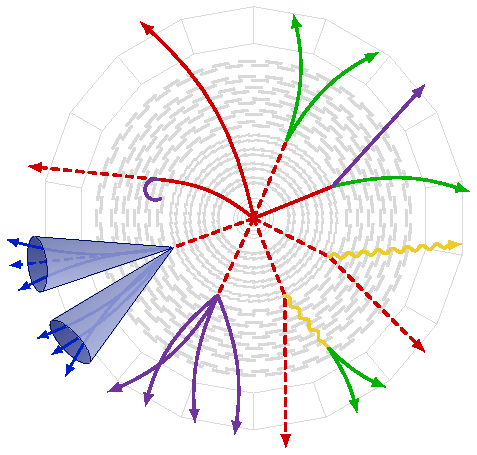
\includegraphics[width=0.2\linewidth]{figures/chapter-01/Collision.pdf}
};


% ------------------------------------------------------------------------
% DETECTOR LEVEL NODES (within detectorBox)
% ------------------------------------------------------------------------
% Data (top)
\node[computer={\textbf{Simulation}\\[-1.5ex]\;}]
  (sim) at ([xshift=2cm, yshift=-1.1cm]detectorBox.north west)
  {};

\node[align=center, opacity=0.75] (data) [below=0.65cm of sim, xshift=0cm, inner sep=0pt, 
    label={center:{\shortstack{\large\textbf{Data}}}}]{
    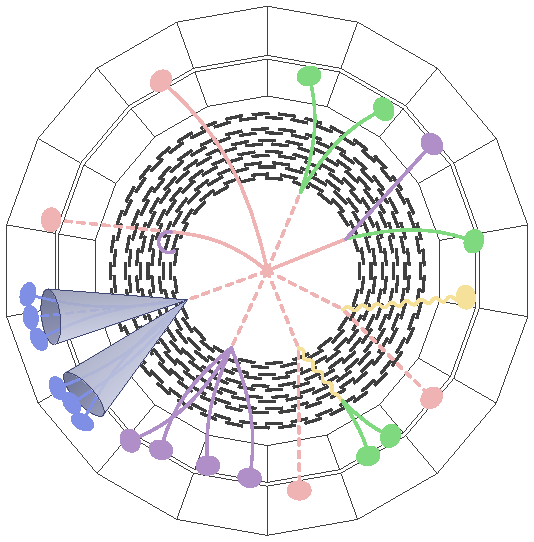
\includegraphics[width=0.2\linewidth]{figures/chapter-01/Collider.pdf}
};




% ------------------------------------------------------------------------
% Connect the re-weighted generation to re-weighted simulation
% (Emulated detector arrow)
% ------------------------------------------------------------------------
\draw[arrowstyle] (gen.east) to
  node[above, align=center, sloped, font=\footnotesize, xshift=0cm, ]{\textbf{\normalsize{Detector}}}
  node[below, align=center, font=\footnotesize, xshift=0cm]{\textbf{Simulation}}
  (sim.west);

\draw[arrowstyle] (truth.east) to
  node[above, align=center, sloped, font=\footnotesize]{\textbf{\normalsize{Detector}}}
  (data.west);

\end{tikzpicture}